% scale_lanes deck: default load balancing — each tier balances on its own.
\documentclass[tikz,border=4pt]{standalone}
\usepackage{fontspec}
\setmainfont{DejaVu Sans}
\setmonofont{DejaVu Sans Mono}
\usetikzlibrary{positioning,arrows.meta,fit,backgrounds,calc,decorations.pathreplacing}
\definecolor{slime}{RGB}{230,230,230}
\definecolor{host}{RGB}{214,216,240}
\definecolor{gpu}{RGB}{255,236,204}
\definecolor{vm}{RGB}{214,238,220}
\definecolor{ac}{RGB}{255,246,230}
\definecolor{bad}{RGB}{245,205,205}
\definecolor{ink}{RGB}{40,40,90}
\begin{document}
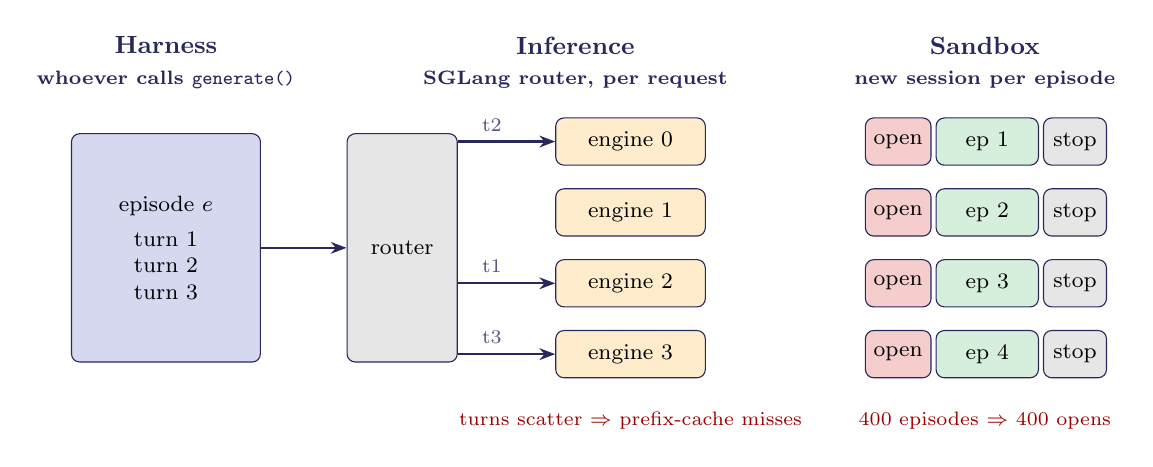
\begin{tikzpicture}[
  font=\footnotesize,
  box/.style={draw=ink, rounded corners=3pt, fill=#1, align=center, inner sep=3pt, minimum height=0.7cm, minimum width=2.2cm},
  line/.style={thick, draw=ink, -{Stealth[length=2mm]}},
  head/.style={font=\small\bfseries, text=ink, align=center},
  note/.style={font=\scriptsize, text=ink!80, align=center},
]
\node[head] at (0,1.0) {Harness\\\scriptsize whoever calls \texttt{generate()}};
\node[head] at (5.2,1.0) {Inference\\\scriptsize SGLang router, per request};
\node[head] at (10.4,1.0) {Sandbox\\\scriptsize new session per episode};
\node[box=host, minimum height=2.9cm, minimum width=2.4cm] (h) at (0,-1.35) {episode $e$\\[3pt]turn 1\\turn 2\\turn 3};
\node[box=slime, minimum width=1.4cm, minimum height=2.9cm] (r) at (3.0,-1.35) {router};
\foreach \i/\y in {0/0,1/-0.9,2/-1.8,3/-2.7} \node[box=gpu, minimum width=1.9cm, minimum height=0.6cm] (e\i) at (5.9,\y) {engine \i};
\draw[line] (h) -- (r);
\draw[line] (r.east |- e2) -- node[above, note, pos=0.35] {t1} (e2);
\draw[line] (r.east |- e0) -- node[above, note, pos=0.35] {t2} (e0);
\draw[line] (r.east |- e3) -- node[above, note, pos=0.35] {t3} (e3);
\node[note, text=red!60!black] at (5.9,-3.55) {turns scatter $\Rightarrow$ prefix-cache misses};
\foreach \k/\y in {1/0,2/-0.9,3/-1.8,4/-2.7} {
  \node[box=bad, minimum width=0.8cm, minimum height=0.6cm] (o\k) at (9.3,\y) {open};
  \node[box=vm, minimum width=1.3cm, minimum height=0.6cm, right=0.05cm of o\k] (v\k) {ep \k};
  \node[box=slime, minimum width=0.8cm, minimum height=0.6cm, right=0.05cm of v\k] {stop};
}
\node[note, text=red!60!black] at (10.4,-3.55) {400 episodes $\Rightarrow$ 400 opens};
\end{tikzpicture}
\end{document}
